\section{A Probabilistic Model of Feature Selection}

%Feature selection is the selection of a subset of features $F^*$ from
%the complete feature space $F,$ for a specific
%classification/prediction problem, without loosing too much
%performance on some given measures. The benefit of feature selection
%include more explainable model, reduced computation time/power, and
%the avoidance of overfitting.
%
%Existing feature selection algorithms, whose performance show no
%statistical difference on out benchmark, are mostly ad-hoc. They give
%various answers to optimisation, but none of them gives the
%question. In this project, we started from the first principles,
%proposed a graphical model, and built a new feature selection system
%upon it.

%\subsection{Graphical Model}

In our work, we wish to derive a model of feature selection in the
filtering framework that focuses specifically on recall (we assume the
classifier itself aims to maximize accuracy or some surrogate).  To
begin our derivation, we propose a graphical model of feature
selection for the binary classification problem, as shown in
Figure~\ref{fig:model}. Double-walled nodes represent observed
variables, including the data point vector $\vec{x}^{d},$ selected
features $f_i^*$ (where $1\leq i\leq k,$ $f_i\in F$) and the
supervised class label $y^d$. Single-walled circle nodes represent
latent variables, including a selected attribute of data
point vector $f_i^x$ (i.e., the value resulting from applying
a deterministic feature function $f_i$ to data input $\vec{x}$) and
the prediction from a feature $y^d_i \in \{0,1\}$ (whose conditional
probability is the maximum likelihood estimate w.r.t.\ the data $D$).
The only part of this model that we have not yet specified is 
$P(y^d|\{y^d_i\})$ which determines how an observed classification 
prediction $y^d$ is made given the latent predictions $y^d_i$ of each 
selected feature $f_i$.  We use a deterministic voting scheme
to represent this conditional probability, which we will discuss
in-depth shortly.  First we focus on selecting features which optimize
this model given some $P(y^d|\{y^d_i\})$.

Since jointly optimizing this objective is NP-hard, we build
$F^*$ in a greedy manner by choosing the next optimal feature $f^*_k$
given the previous set of optimal features $F^*_{k-1}$ and recursively
defining $F^*_k = F^*_{k-1}\cup f^*_k$ with $F^*_0 = \emptyset$. The
fitness measure of a selected feature set $F^*_k$ can be
expressed in terms of log or expected likelihood, discussed next.

\begin{figure}[tbp!]
	\centering
	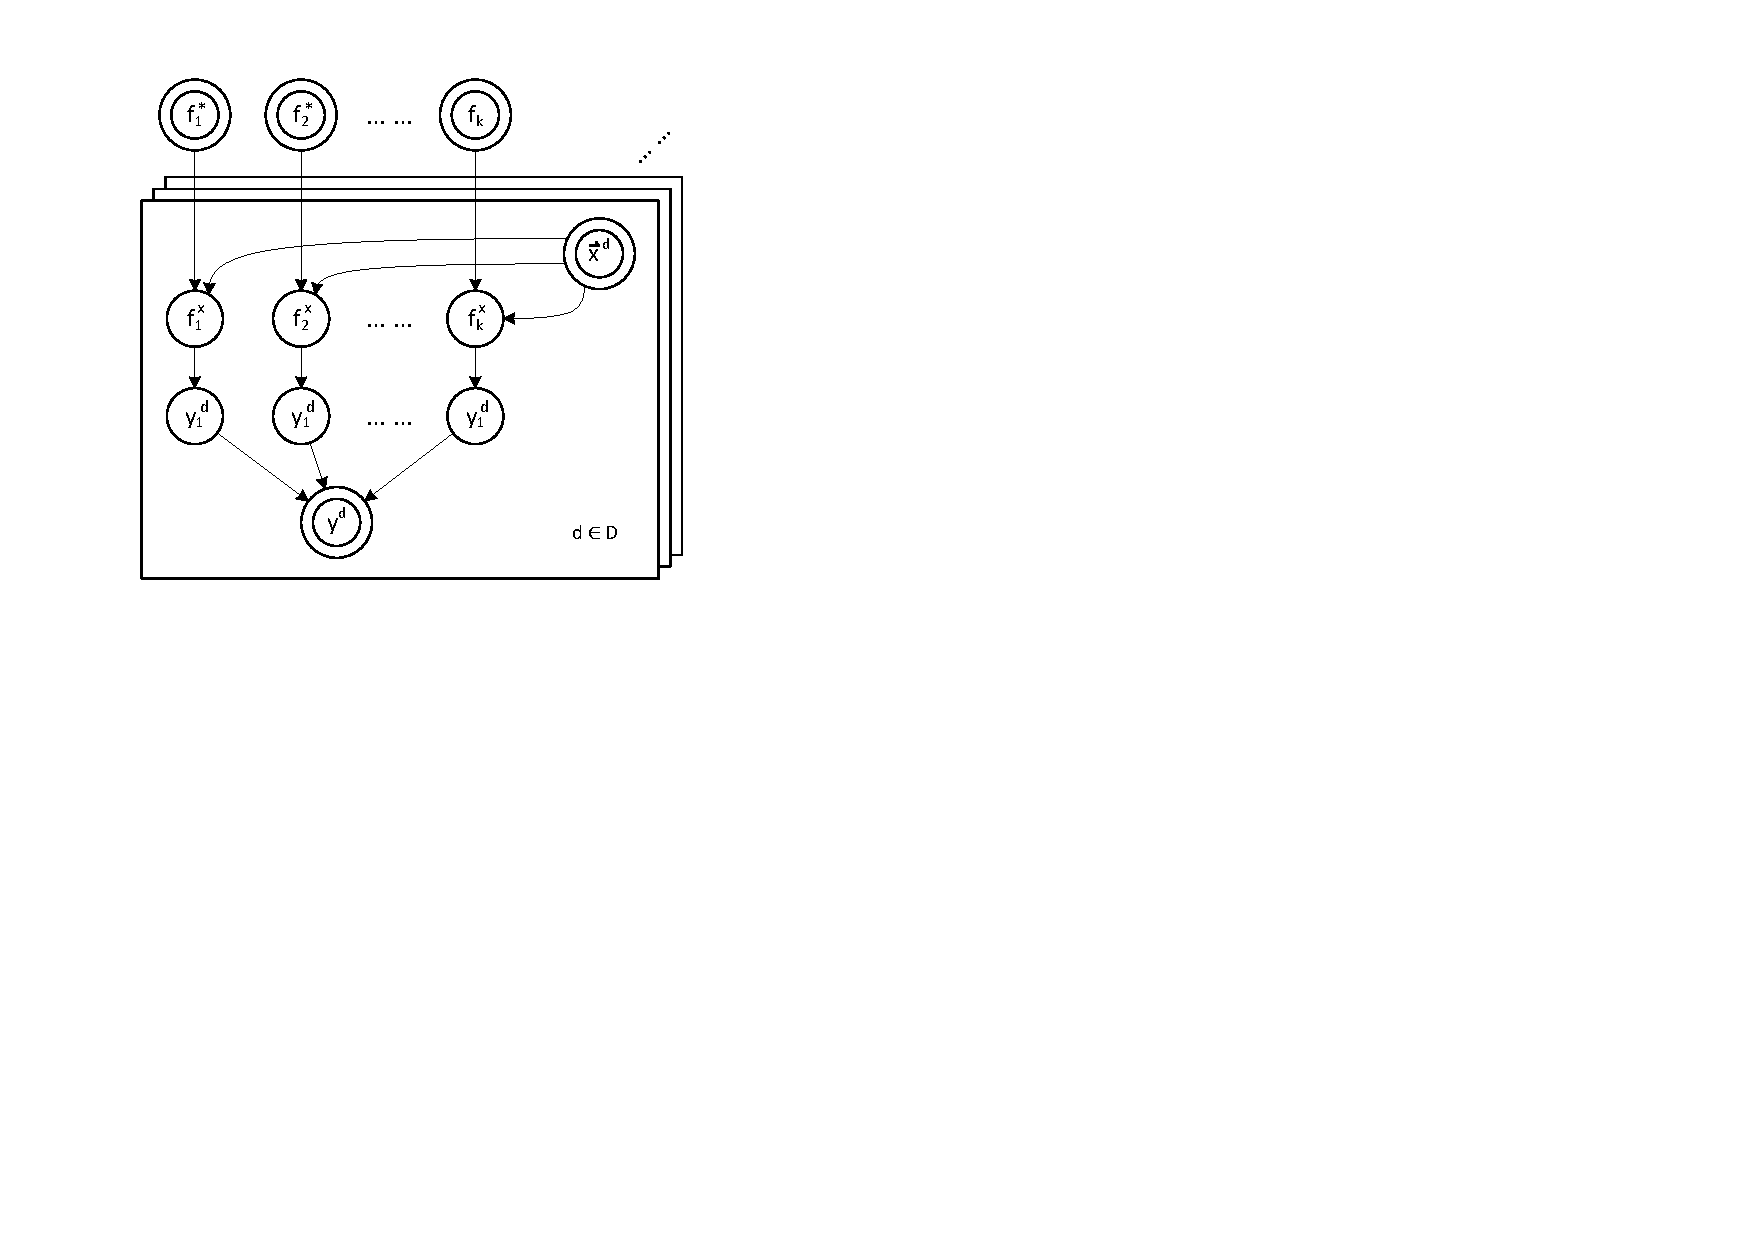
\includegraphics[scale=0.9]{Plots_1.pdf}
	\caption{\footnotesize A probabilistic voting model of classification represented as a graphical model. 
Double-walled circles denote observed nodes, single-walled circles denote latent (unobserved) nodes.}
	\label{fig:model}
\end{figure}

%\subsection{Objective}

\COMMENT
\subsubsection{Expected Likelihood}
The initial objective is defined as:
\[f_k^*=\argmax_{f_k}E_D\left[P\left(y^d|\vec{x}^{\,d},F_k\right)\right]\]

{\small
\begin{align}
f_k^*&=\argmax_{f_k}E_D\left[P\left(y^d|\vec{x}^{\,d},F_k\right)\right]\nonumber\\
&=\argmax_{f_k}\frac{1}{|D|}\sum_{d\in D} P\left(y^d | \vec{x}^{\,d},F_k\right)\nonumber\\
&=\argmax_{f_k}\sum_{d\in D}\frac{P\left(y^d,\vec{x}^{\,d},F_k\right)}{P\left(\vec{x}^{\,d},F_k\right)}\nonumber\\
&=\argmax_{f_k}\sum_{d\in D}\sum_{\{y_{i}^d\}_{1\leq i\leq k}}\frac{P\left(y^d,\vec{x}^{\,d},F_k,\{y_{i}^d\}_{1\leq i\leq k}\right)}{P\left(\vec{x}^{\,d},F_k\right)}\nonumber\\
%=\argmax_{f_k}&\sum_{d \in D}\sum_{{\{y_{i}^d\}}_{1\leq i\leq k}}\frac{P\left(y^d|\{y^d_i\}_{1\leq i\leq k}\right)\left(\prod_{i=1}^kP\left(y_i^d|\vec{x}^{\,d}, f_i\right)\right)P\left(\vec{x}^{\,d}\right)\prod_{i=1}^kP\left(f_i\right)}{P\left(\vec{x}^{\,d},F_k\right)}\nonumber\\
&=\argmax_{f_k}\sum_{d\in D}\sum_{\{y_i^d\}_{1\leq i\leq k}}P\left(y^d|\{y^d_i\}_{1\leq i\leq k}\right)\prod_{i=1}^kP\left(y_i^d|\vec{x}^{\,d},f_i\right)\label{eq:expect}
\end{align}}

Here, we rewrote the expectation of a binary event as its probability,
factorized the conditional probability in the joint probability
divided by the marginal, marginalised over $\{y^d_i\}_{1\leq i\leq
  k}$, factorized joint probability in conditional and prior following
the graphical model and exploited d-separation to remove irrelevant
conditions and to cancel terms in the equation.

Now we can optimise our initial objective aiming three goals of classification tasks: Precision, Recall, and General n-out-of-k.
\ENDCOMMENT

\paragraph{Log Likelihood (L)}

Because Figure~\ref{fig:model} essentially provides a probabilistic classifier model as a function
of the input data and selected features, we can choose features so as to maximize the log likelihood
of the data given the model (i.e., features selected), i.e., $l(D|F_k^*)$ as follows:

{\small 
\begin{align}
f_k^*&=\argmax_{f_k} l(D|F^*_k) \nonumber
\end{align}
\begin{align}
&=\argmax_{f_k}\,\log\prod_{d\in D}P\left(y^d|\vec{x}^{\,d},F_k\right)\nonumber\\
&=\argmax_{f_k}\sum_{d\in D}\log\left(\frac{P\left(y^d,\vec{x}^{\,d},F_k\right)}{P\left(\vec{x}^{\,d},F_k\right)}\right)\nonumber \\
&=\argmax_{f_k}\sum_{d\in D}\log \!\!\! \sum_{\{y_i^d\}_{1\leq i\leq k}} \!\!\! \frac{P\left(y^d,\vec{x}^{\,d}, F_k,\{y_i^d\}_{1\leq i\leq k}\right)}{P\left(\vec{x}^{\,d},F_k\right)}\nonumber\\
%&=\argmax_{f_k} \sum_{d \in D} \log\sum_{{\{y_i^d\}}_{1\leq i \leq k}} \frac{P\left(y^d| \{y^d_i\}_{1 \leq i \leq k}\right) \prod_{i=1}^kP\left(y_i^d|\vec{x}^{\,d},f_i\right)P\left(\vec{x}^{\,d}\right)\prod_{i=1}^kP\left(f_i\right)}{P\left(\vec{x}^{\,d}, F_k\right)}\nonumber\\
&=\argmax_{f_k}\sum_{d\in D}\log \!\!\! \sum_{{\{y_i^d\}}_{1\leq i\leq k}} \!\!\! P\left(y^d|\{y^d_i\}_{1\leq i\leq k}\right) \prod_{i=1}^kP\left(y_i^d|\vec{x}^{\,d},f_i\right) \label{eq:expect} 
\end{align}}

Here, we rewrote the likelihood of a binary event as its probability,
factorized the conditional probability in the joint probability
divided by the marginal, marginalized over $\{y^d_i\}_{1\leq i\leq
  k}$, factorized joint probability in conditional and prior following
the graphical model and exploited D-separation to remove irrelevant
conditions and to cancel terms in the equation.

\paragraph{Expected Likelihood (E)}

In contrast to log likelihood which tends to give more weight to extreme
probabilities, we may wish to instead maximize expected likelihood
defined as follows:
\begin{align*}
f_k^*&=\argmax_{f_k}E_D\left[P\left(y^d|\vec{x}^{\,d},F_k\right)\right]\nonumber\\
&=\argmax_{f_k}\frac{1}{|D|}\sum_{d\in D} P\left(y^d | \vec{x}^{\,d},F_k\right)\nonumber\\
&=\argmax_{f_k} \sum_{d\in D} P\left(y^d | \vec{x}^{\,d},F_k\right)\nonumber\\
\end{align*}
If we remove the logarithm from the previous derivation above, we easily
derive the final result of the log likelihood in~\eqref{eq:expect} without the $\log$.

%Since $\sum_{d\in D}log\sum_{{\{y_i^d\}}_{1\leq i\leq
%    k}}P\left(y^d|\{y^d_i\}_{1\leq i\leq
%  k}\right)\prod_{i=1}^kP\left(y_i^d|\vec{x}^{\,d},f_i\right)$ is
%exactly the same as the result in the expectation case, and the
%logarithm is a monotonous function, the choice of likelihood instead
%of expectation has no further affect on the algorithm.

\paragraph{Voting Schemes for High Recall}

Critically, it is how we specify the model and objective that we
believe should encourage feature selection with high recall.
Specifically, we have complete license in Figure~\ref{fig:model} to
determine the conditional probability $P(y^d|\{y^d_i\})$, which
represents how the class prediction $y_d$ is determined from the class
prediction of each feature denoted as $y^d_i$.  Here we consider two
different extreme voting schemes represent logical conjuntion and
disjunction of the feature votes (defined shortly).  If we use
conjunction, we require strong agreement among all features for a
datum to be classified as true while for the disjunctive case, only
one feature need vote true for the classification to be true.
Overall, we believe conjunctive is better in terms of cancelling
effects of noisy features (hence leading to accuracy), but we derive
the results for both conjunction and disjunction since they are
symmetric and will allow us to test this hypothesis.  We remark that a
critical feature of our two objectives above based on log and expected
likelihood is that each datum is weighted equally and the newly
selected features $f_k^*$ which leads to more correct classifications
for more data (especially those not already classified correctly under
the model of Figure~\ref{fig:model}) are more likely to be selected,
hence overall targeted recall.

\paragraph{Conjunctive Voting (CV)}
In order to select the subset of features with conjunctive voting, 
we need the agreement of all features predictors
$y^d_i$ to predict true. That is, when $y^d$ is true we need all of
the predictors $y^d_i$ equals to true, and if $y^d$ were false, just
one of the predictors $y^d_i$ would have to be false. Then the
probability $P\left(y^d|\{y^d_i\}_{1\leq i\leq k}\right)$ can be
expressed as follows:
{\small 
\begin{align}
P\left(y^d|\{y^d_i\}_{1\leq i\leq k}\right) & =I\left[y^d=\bigwedge_{i=1}^k y^d_i\right] \nonumber\\
&= \begin{cases}
	y^d=1 \text{ when } \{y_i^d=1\}_{1\leq i\leq k}\\
	y^d=0 \text{ when } \{y_i^d\}_{1\leq i\leq k,\exists{y_j^d\|y_j^d=0}}
\end{cases}\label{eq:expect_pre_1}
\end{align}}
Then, we combined equations \eqref{eq:expect} and
\eqref{eq:expect_pre_1}, separated each term according to the actual
label value $y^d$ and used the probability sum rule to rewire the
second term as follows:
\begin{align}
f_k^*&=\argmax_{f_k}\sum_{d\in D}I\left[y^d=\bigwedge_{i=1}^k y^d_i\right]\prod_{i=1}^kP\left(y_i^d|\vec{x}^{\,d},f_i\right)\nonumber\\[0.5em]
&=\argmax_{f_k}\sum_{d\in D}
\begin{cases}
	y^d=1: \prod_{i=1}^kP\left(y_i^d=1|\vec{x}^{\,d},f_i\right)\\
	y^d=0: \sum_{\substack{\{y_i^d\}_{1\leq i\leq k},\\ \exists{y_i^d\|y_i^d=0}}}\prod_{i=1}^kP\left(y_i^d|\vec{x}^{\,d},f_i\right)
\end{cases}\nonumber\\[0.5em]
&=\argmax_{f_k}\sum_{d\in D}
\begin{cases}
	y^d=1: \prod_{i=1}^kP\left(y_i^d = 1|\vec{x}^{\,d},f_i\right)\\
	y^d=0: 1-\prod_{i=1}^kP\left(y_i^d = 1|\vec{x}^{\,d},f_i\right)
\end{cases}\label{eq:expect_pre_2}\\[0.5em]
&=\argmax_{f_k}\sum_{d\in D}
\begin{cases}
	y^d=1: \prod_{i=1}^kP\left(y^d = 1|\vec{x}_i^{\,d},f_i\right)\\
	y^d=0: 1-\prod_{i=1}^kP\left(y^d = 1|\vec{x}_i^{\,d},f_i\right)\nonumber
\end{cases}
\end{align}
From \eqref{eq:expect_pre_2} we can intuitively describe how this
equation is related to the precision metric. In the confusion matrix,
Precision is calculated dividing the numbers of true positives by the
number of all examples predicted as positive (true positives and false
positives). When $y^d$ is true, \eqref{eq:expect_pre_2} gives higher
score to feature that have higher probability to predict true,
encouraging true positives. Meanwhile, if $y^d$ is false,
\eqref{eq:expect_pre_2} gives lower score to features that have higher
probability to predict true, penalising false positives.

\paragraph{Disjunctive Voting (DV)}
In order to select the subset of features with disjunctive voting,
we need at least one $y^d_i$ to predict true. Therefore, we
need a disjunction operation between the predictors $y^d_i$. That is,
when $y^d$ is true, we need at least one predictor $y^d_i$ to equals
to true, and if $y^d$ were false, all of the predictors $y^d_i$ would
have to be false. Then the probability $P\left(y^d|\{y^d_i\}_{1\leq
  i\leq k}\right)$ can be expressed as follows:
{\small 
\begin{align}
P\left(y^d|\{y^d_i\}_{1\leq i\leq k}\right) & =I\left[y^d=\bigvee_{i=1}^k y^d_i\right] \nonumber \\
& = \begin{cases}
	y^d=1 \text{ when } \{y_i^d\}_{1\leq i\leq k,\exists{y_j^d\|y_j^d=1}}\\
	y^d=0 \text{ when } \{y_i^d=0\}_{1\leq i\leq k}
\end{cases}\label{eq:expect_recall_1}
\end{align}}
Here, we combined equations \eqref{eq:expect} and
\eqref{eq:expect_recall_1}, separated each term according to the
actual label value $y^d$ and used the probability sum rule to rewrite
the second term as follows:
\begin{align}
f_k^*&=\argmax_{f_k}\sum_{d\in D}I\left[y^d=\bigvee_{i=1}^k y^d_i\right]\prod_{i=1}^kP\left(y_i^d|\vec{x}^{\,d},f_i\right)\nonumber\\[0.5em]
&=\argmax_{f_k}\sum_{d\in D}
\begin{cases}
	y^d=0: \prod_{i=1}^kP\left(y_i^d=0|\vec{x}^{\,d},f_i\right)\\
	y^d=1: \sum_{\substack{\{y_i^d\}_{1\leq i\leq k},\\ \exists{y_i^d\|y_i^d=1}}}\prod_{i=1}^kP\left(y_i^d|\vec{x}^{\,d},f_i\right)
\end{cases}\nonumber\\[0.5em]
&=\argmax_{f_k}\sum_{d\in D}
\begin{cases}
	y^d=0: \prod_{i=1}^kP\left(y_i^d=0|\vec{x}^{\,d},f_i\right)\\
	y^d=1: 1-\prod_{i=1}^kP\left(y_i^d=0|\vec{x}^{\,d},f_i\right)
\end{cases}\label{eq:expect_recall_2}\\
&=\argmax_{f_k}\sum_{d\in D}
\begin{cases}
	y^d=0: \prod_{i=1}^kP\left(y^d=0|\vec{x}_i^{\,d},f_i\right)\\
	y^d=1: 1-\prod_{i=1}^kP\left(y^d=0|\vec{x}_i^{\,d},f_i\right)
\end{cases}\nonumber
\end{align}
From \eqref{eq:expect_recall_2} we can intuitively describe how this
equation is related to the precision metric. In the confusion matrix,
Recall is calculated dividing the numbers of actual true positives by
the number of all true positives (true positives and false
negatives). When $y^d$ is false, \eqref{eq:expect_recall_2} gives
higher score to feature that have higher probability to predict false,
encouraging true negatives. Meanwhile, if $y^d$ is true,
\eqref{eq:expect_recall_2} gives lower score to features that have
higher probability to predict false, penalizing false negatives.

